\section{Method}

\subsection{Noising as partial masking}
Recall that \emph{masking} is the practice of occluding a subset of data, such as patches of an image~\cite{he2022masked} or timesteps in a sequence~\cite{bert, t5}, and training a model to recover unmasked portions. 
Without loss of generality, we can view any collection of tokens, sequential or not, as an ordered set indexed by $t$.
Training next-token prediction with teacher forcing can then be interpreted as masking each token $\bx_t$ at time $t$ and making predictions from the past  $\bx_{1:t-1}$. Restricted to sequences, we refer to all these practices as \emph{masking along the time axis}. We can also view full-sequence forward diffusion, i.e., gradually adding noise to the data $ \bx^0_{1:T} \equiv \bx_{1:T}$, as a form of \emph{partial masking}, which we refer to as \emph{masking along the noise axis}. Indeed, after $K$ steps of noising, $\bx^K_{1:T}$ is (approximately) pure white noise without information about the original data.

We establish a unified view along both axes of masking (see Fig.~\ref{fig:method}).  We denote  $\bx_{1:T}$ for a sequence of tokens, where the subscript indicates the time axis. As above, $\xtk$ denotes $\bx_t$ at noise level $k_t$ under the forward diffusion process~\eqref{eqn:forward_diffusion};  $\bx_t^0 = \bx$ is the unnoised token, and  $\bx^K_t$ is white noise $ \mathcal{N}(0, \mathbf{I})$. Thus, $(\xtk)_{1 \le t \le T}$ denotes a sequence of noisy observations where each token has a \emph{different} noise level $k_t$, which can be seen as the degree of \emph{partial masking} applied to each token through noising.

\subsection{\algons{}: different noise levels for different tokens}
\emph{\algo{}} ({\algshort}) is a framework for training and sampling arbitrary sequence lengths of noisy tokens $(\xtk)_{1 \le t \le T}$, where critically, \emph{the noise level $k_t$ of each token can vary by time step}. 
In this paper, we focus on time series data, and thus instantiate \algo{} with causal architectures (where $\xtk$ depends only on past noisy tokens), which we call \emph{\algoseq{}} ({\algshortseq{}}).
For simplicity, we focus on a minimal implementation with a vanilla Recurrent Neural Network (RNN) ~\cite{gru}. Potential transformer implementation of \algo{} is also possible but we defer its discussion to Appendix~\ref{app:transformer}.

\begin{figure}[t]
  \begin{minipage}[t]{0.5\linewidth}
    \centering
    \footnotesize
    \begin{algorithm}[H]
\footnotesize
\caption{\algo{} Training}
\label{alg:diffusion_forcing_training}
\begin{algorithmic}[1]
\LOOP
    \STATE Sample tajectory of observations $(\bx_1, ..., \bx_T)$.
    \FOR{$t = 1, ..., T$}
        \STATE Sample independent noise level $k_t \in \{0,1, ... ,K\}$
        \STATE $\xtk=\ $ForwardDiffuse$(\bx_t, k_t)$
        \STATE Define $\epsilon_t = \frac{\xtk-\sqrt{\bar{\alpha}_{k_t}} \bx_t}{\sqrt{1-\bar{\alpha}_{k_t}}}$ 
         \STATE Update $\bz_t \sim p_\theta(\bz_t|\bz_{t-1}, \xtk, k_t)$.
        \STATE Set $\hat{\epsilon}_t = \epsilon_\theta(\bz_{t-1},\xtk,k_t)$
    \ENDFOR
    \STATE $L=$MSELoss$(\left[\hat{\epsilon}_1, ..., \hat{\epsilon}_n\right], \left[\epsilon_1, ..., \epsilon_n\right])$ 
    \STATE Backprop with $L$ and update $\theta$
\ENDLOOP
\end{algorithmic}
\end{algorithm}

  \end{minipage}
  \hfill
  \begin{minipage}[t]{0.5\linewidth}
    \centering
    \footnotesize
    \section{Sampling observations in \textsc{diamond}}
\label{appendix:sampling}

We describe here how we sample an observation $\x_t^0$ from our diffusion world model. We initialize the procedure with a noisy observation $\x_t^\Tau \sim p^{prior}$, and iteratively solve the reverse SDE in Equation \ref{eq:reverse_process} from $\tau = \Tau$ to $\tau = 0$, using the learned score model $\mathbf{S}_\theta(\x_t^\tau, \tau, \x_{<t}^0, a_{<t})$ conditioned on past observations $\x_{<t}^0$ and actions $a_{<t}$. This procedure is illustrated in Figure \ref{fig:architecture}.

In fact, there are many possible sampling methods for a given learned score model $\mathbf{S}_\theta$ \citep{karras2022elucidating}. Notably, \citet{song_sde} introduce a corresponding ``probability flow" ordinary differential equation (ODE), with marginals equivalent to the stochastic process described in Section \ref{subsec:diffusion}. In that case, the solving procedure is deterministic, and the only randomness comes from sampling the initial condition. In practice, this means that for a given score model, we can resort to any ODE or SDE solver, from simple first order methods like Euler (deterministic) and Euler–Maruyama (stochastic) schemes, to higher-order methods like Heun's method \citep{ascher1998computer}. 

Regardless of the choice of solver, each step introduces truncation errors, resulting from the local score approximation and the discretization of the continuous process. Higher order samplers may reduce this truncation error, but come at the cost of additional Number of Function Evaluations (NFE) -- how many forward passes of the network are required to generate a sample. This local error generally scales superlinearly with respect to the step size (for instance Euler's method is $\mathcal{O}(h^2)$ for step size $h$), so increasing the number of denoising steps improves the visual quality of the generated next frame. Therefore, there is a trade-off between visual quality and NFE that directly determines the inference cost of the diffusion world model.


% with t+1 instead of t

% \section{Sampling next observations in \textsc{diamond}}
% \label{appendix:sampling}

% We describe here how we sample a next observation $\x_{t+1}$ from our diffusion world model. We initialize the procedure with a noisy next observation $\x_{t+1}^\Tau \sim p^{prior}$, and iteratively solve the reverse SDE in Equation \ref{eq:reverse_process} from $\tau = \Tau$ to $\tau = 0$, using the learned score model $\mathbf{S}_\theta(\x_{t+1}^\tau, \tau, \x_{\le t}^0, a_{\le t})$ conditioned on past observations $\x_{\le t}^0$ and actions $a_{\le t}$. This procedure is illustrated in Figure \ref{fig:architecture}.

% In fact, there are many possible sampling methods for a given learned score model $S_\theta$ \citep{karras2022elucidating}. Notably, \citet{song_sde} introduce a corresponding ``probability flow" ordinary differential equation (ODE), with equivalent marginals. In that case, the solving procedure is deterministic, and the only randomness comes from sampling the initial condition. In practice, this means that for a given score model, we can resort to any ODE or SDE solver, from simple first order methods like Euler (deterministic) and Euler–Maruyama (stochastic) schemes, to higher-order methods like Heun's method \citep{ascher1998computer}. 

% Regardless of the choice of solver, each step introduces truncation errors, resulting from the local score approximation and the discretization of the continuous process. Higher order samplers may reduce this truncation error, but come at the cost of additional Number of Function Evaluations (NFE) -- how many forward passes of the network are required to generate a sample. This local error generally scales superlinearly with respect to the step size (for instance Euler's method is $\mathcal{O}(h^2)$ for step size $h$), so increasing the number of denoising steps improves the visual quality of the generated next frame. Therefore, there is a trade-off between visual quality and NFE that directly determines the inference cost of the diffusion world model.



  \end{minipage}
  \vspace{-12pt}
\end{figure}


The RNN with weights $\theta$ maintains latents $\bz_t$ capturing the influence of past tokens, and these evolve via dynamics $\bz_t \sim p_{\theta}(\bz_t |  \bz_{t-1}, \xtk, k_t)$ with a recurrent layer. When an incoming noisy observation $\xtk$ is made, the hidden state is updated in a Markovian fashion $\bz_t \sim p_{\theta}(\bz_t | \bz_{t-1}, \xtk, k_t)$\footnote{We implement $\bz_t = p_{\theta}(\bz_t | \bz_{t-1}, \xtk, k_t)$ to be deterministic, with $\bz_t$ representing a distribution over beliefs rather than a sample from it. This allows training by backpropogating through the latent dynamics in Eq.\eqref{eq:train}.}. When $k_t = 0$, this is the posterior update in Bayes filtering; whereas when $k_t = K$ (and $\bx_t^K$ is pure noise and thus uninformative), this is equivalent to modeling the ``prior distribution'' $p_{\theta}(\bz_t \mid \bz_{t-1})$ in Bayes filtering. Given latent $\bz_t$, an observation model $p_{\theta}(\bx_t^0 | \bz_t)$ predicts $\bx_t$.


\paragraph{Training.}
The dynamics model $p_{\theta}(\bz_t |  \bz_{t-1}, \xtk, k_t)$ and the observation model $p_{\theta}(\bx_t^0 | \bz_t)$ together form a RNN unit. Such unit has the same input-output behavior as a standard conditional diffusion model, using a conditioning variable $\bz_{t-1}$ and a noisy token  $\xtk$ as input to predict the noise-free $\bx_t = \bx_t^0$ and thus, indirectly, the noise $\epsilon^{k_t}$ via affine reparametrization \cite{ddpm}. 
We can thus directly train \algopar{} with the conventional diffusion training objective. We parameterize the aforementioned  unit in terms of noise prediction $\beps_{\theta}(\mathbf{z}_{t-1}, \xtk, k_t)$.
We then find parameters $\theta$ by minimizing the loss 
\begin{equation}\label{eq:train}
\mathop{\mathlarger{\mathbb{E}}}_{\substack{k_t, \bx_t, \beps_t \\ \bz_t\sim p_{\theta}(\bz_t|\bz_{t-1},\xtk,k_t)}} {\textstyle \mathlarger{\sum}_{t=1}^T}
\Big[\| \beps_t - \beps_\theta(\bz_{t-1},\xtk,k_t) \|^2\Big],
\end{equation}\vspace{-.1em}%
where we sample $k_{1:T}$ uniformly from $[K]^T$, $\bx_{1:T}$ from our training data, and $\epsilon_t \sim \cN(0,\sigma^2_{k_t} I)$ in accordance with the forward diffusion process (see Algorithm \ref{alg:diffusion_forcing_training}  for pseudocode). Importantly, the loss \eqref{eq:train} captures essential elements of Bayesian filtering and conditional diffusion. 
In Appendix~\ref{app:snr_derivation}, we further re-derive common techniques in diffusion model training for \algo{}, which proves extremely useful for video prediction experiments. In Appendix~\ref{app:independent_noise}, we discuss the need of sampling $k_{1:T}$ uniformly. Finally, we prove the validity of this objective stated informally in the following Theorem~\ref{theorem:informal} in Appendix~\ref{appendix:theory}.
\vspace{2pt}
\begin{theorem}[Informal] The \algo{} training procedure (\Cref{alg:diffusion_forcing_training}) optimizes a reweighting of an Evidence Lower Bound (ELBO) on the expected log-likelihoods $\ln p_{\bm \theta}((\bx_t^{k_t})_{1 \le t \le T})$, where the expectation is averaged over noise levels $k_{1:T} \sim [K]^T$ and $\bx_t^{k_t} $ noised according to the forward process. Moreover, under appropriate conditions, optimizing \eqref{eq:train} also maximizes a lower bound on the likelihood for \emph{all sequences of noise levels, simultaneously}. 
\label{theorem:informal}
\end{theorem}

We remark that a special case of `all sequences of noise levels' are those for which either $k_t = 0$ or $k_t = K$; thus, one can mask out \emph{any prior token} and \algshort{} will learn to sample from the correct conditional distribution, modeling the distribution of all possible sub-sequences of the training set. 


\paragraph{Sampling.}
\label{sec:zigzag_example}
\algo{} sampling is depicted in \Cref{alg:diffusion_forcing_sampling}  and is defined by prescribing a noise schedule on a 2D $M \times T$ grid $\cK \in [K]^{M\times T}$; columns correspond to time step $t$ and rows indexed by $m$ determine noise-level. $\cK_{m,t}$ represents the desired noise level of the time-step $t$ token for row $m$.  
To generate a whole sequence of length $T$,  initialize the tokens $\bx_{1:T}$ to be white noise, corresponding to noise level $k = K$. We iterate down the grid row-by-row, denoising left-to-right across columns to the noise levels prescribed by $\cK$. By the last row $m = 0$, the tokens are clean, i.e. their noise level is $\cK_{0,t} \equiv 0$. \Cref{app:corner_case} discusses corner cases of this scheme; the  hyperparameters $(\alpha_k,\bar{\alpha}_k,\sigma_k)$ are set to their standard values \cite{ddpm}. The matrix $\cK$ specifies how fast each token gets denoised at every step of sequence diffusion. Since \algo{} is trained to denoise tokens of all sequences of noise levels, $\cK$ can be designed to flexibly achieve different behaviors without re-training the model. 






\subsection{New Capabilities in Sequence Generation}
We now explain the new capabilities this flexible sampling paradigm has to offer. 

\begin{figure*}[h]
    \centering
    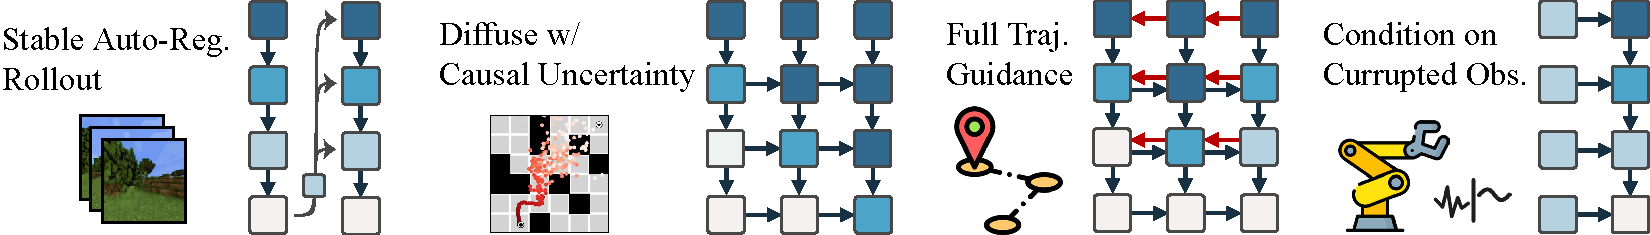
\includegraphics[width=\linewidth]{figures/pdf/Sampling_Schemes.pdf}
    \vspace{-10pt}
\end{figure*}


\paragraph{Stabilizing autoregressive generation.}
\label{par:stabilizing_autoreg}
For high-dimensional, continuous sequences such as video, auto-regressive architectures are known to diverge, especially when sampling past the training horizon.
In contrast, \algo{} can stably  roll out long sequences even beyond the training sequence length by updating the latents using the previous latent associated with  slightly ``noisy tokens'' for some small noise level $0 < k \ll K$. Our experiments (Sec.~\ref{exp:video}) illustrates the resulting marked improvements in long-horizon generation capabilities;  App. \ref{app:noising_long_horizons} provides further intuition.

\paragraph{Keeping the future uncertain.} 
\label{par:zigzag}
Beginning from a sequence of white noise tokens $[\bx^K_1,\bx^K_2,\bx^K_3]^\top$, we may denoise the first token fully and the second token partially, yielding $[\bx^0_1,\bx^{K/2}_2,\bx^K_3]^\top$, then $[\bx^0_1,\bx^{0}_2,\bx^{K/2}_3]^\top$, and finally denoising all tokens fully to $[\bx^0_1,\bx^0_2,\bx^0_3]^\top$. 
Interpreting the noise level as uncertainty, this ``zig-zag'' sampling scheme intuitively encodes the immediate future as more certain than the far future. Sec.~\ref{sec:method_decision_making} describes how this leads to more effective sequence guidance.

\paragraph{Long-horizon Guidance.}
In Line 10 of Algorithm~\ref{alg:diffusion_forcing_sampling}, one may add guidance to the partially diffused trajectory $\bx_{1:T}$ as in Sec.~\ref{sec:related_prelim}. Due to the dependency of future tokens on the past, guidance gradients from future tokens can propagate backwards in time. The unique advantage of \algo{} is that, because we can diffuse future tokens without fully diffusing the past, the gradient guides the sampling of \emph{past} tokens, thereby achieving long-horizon guidance while respecting causality. We elaborate on implementation details in Appendix ~\ref{app:reward_guidance}. As we  show in \Cref{sec:exp_decision_making}, planning in this manner significantly outperforms guided full-sequence diffusion models.

\subsection{\algo{} for Flexible Sequential Decision Making}
\label{sec:method_decision_making}
The capabilities offered by \algo{} motivate our novel framework for sequential decision making (SDM), with key applications to  robotics and autonomous agents. 
Consider a Markov Decision Process defined by an environment with dynamics $ p(\bs_{t+1}|\bs_t, \ba_t)$, observation $ p(\bo_{t}|\bs_t)$ and reward $p(\br_t|\bs_t, \ba_t)$. The goal is to train a policy $\pi(\ba_t|\bo_{1:t})$ such that the expected cumulative reward of a trajectory $\Exp[\sum_{t=1}^{T} \br_t]$ is maximized. 
We assign tokens $\bx_t = [\ba_t, \br_t, \bo_{t+1}]$.  A trajectory is a sequence $\bx_{1:T}$, possibly of variable length;  training is conducted as in Algorithm \ref{alg:diffusion_forcing_training}. 
At each step $t$ of execution, past (noise-free) tokens $\bx_{1:t-1}$ are  summarized by a latent $\bz_{t-1}$.  Conditioned on this latent, we sample, via Algorithm \ref{alg:diffusion_forcing_sampling}, a plan $\hat{\bx}_{t:t+H}$, with $\hat{\bx}_{t}=[\hat{\ba}_t, \hat{\br}_t, \hat{\bo}_{t+1}]^\top$ containing predicted actions, rewards and observations. $H$ is a look-ahead window, analogous to future predictions in model predictive control \cite{garcia1989model}. After taking planned action $\hat{\ba}_t$, the environment produces a reward $\br_t$ and next observation $\bo_{t+1}$, yielding  next token $\bx_t=[\hat{\ba}_t, \br_t, \bo_{t+1}]^\top$. The latent is updated according to the posterior $p_\theta(\bz_{t}|\bz_{t-1}, \bx_t, 0)$. Our framework enables functionality as both \emph{policy} and \emph{planner}:


\paragraph{Flexible planning horizon.} \algons{} (a) can be deployed on \emph{tasks of variable horizon}, because each new action is selected sequentially, and  
(b) its lookahead window $H$ can be shortened to lower latency (using \algo{} as a \emph{policy}), or lengthened to perform long-horizon \emph{planning} (via guidance described below), without re-training or modifications of the architecture. Note that (a) is not possible for full-sequence diffusion models like Diffuser \cite{janner2022planning} with full-trajectory generation horizons, whereas diffusion policies \cite{chi2023diffusion} need fixed, small lookahead sizes, precluding (b). 


\paragraph{Flexible reward guidance.} As detailed in Appendix~\ref{app:reward_guidance},
\algo{} can plan via guidance using any reward (in place of $\log c$) specified over future steps: this includes dense per-time step rewards on the entire trajectory $\sum_{t=1}^T \br_t$, dense rewards on a future lookahead $\sum_{t'=t}^{t+H}\br_t$, and sparse rewards indicating goal completion $-\|\bo_T-\mathbf{g}\|^2$. Per-time step policies cannot take advantage of this latter, longer horizon guidance. 














  



\paragraph{Monte Carlo Guidance (MCG), future uncertainty.}
\algoseq{} allows us to influence the generation of a token $\mathbf{x}_t^k$ by guidance on the whole distribution of future $\mathbf{x}_{t+1:T}$. Instead of drawing a single trajectory sample to calculate this guidance gradient, we can draw multiple samples of the future and average their guidance gradients. We call this Monte Carlo Guidance. In the spirit of so-called shooting methods like MPPI \cite{ williams2015model}, $\mathbf{x}_t^k$ is then guided by the expected reward over the distribution of all future outcomes instead of one particular outcome.  The effect of MCG is enhanced when combined with sampling schedules that keep the noise level of future tokens high when denoising immediate next tokens (e.g. the zig-zag schedule described in Sec.~\ref{par:zigzag}), accounting for greater uncertainty farther into the future. Appendix~\ref{app:cannot_mcg} further justifies the significance of MCG, and why \algo{}  uniquely takes  advantage of it.






